\chapter{Natural Language Processing}\label{ch_nlp}
\chapterauthor{Ellis Cain}

\textit{Some introduction: Natural language processing has seen an increase in public attention with the recent batch of advanced large language models (LLMs), with the release of GPT4 and LLaMA(?)\footnote{These will probably be surpassed soon.}. It is helpful to first understand the history and context of the field, before moving on to more complex models.}


\textit{Description of the question of the field: how can we process text to extract meaningful information from it? Given a set of documents, how can we find the most relevant search term? How can we computationally evaluate or measure the semantics of words?}

Early on, there were some simple approaches that were manual or math-based(?).

- Manual feature vectors.  Example: the 6 bit vectors in Elman's ``Finding structure in time''

- One-hot codings as a very simple approach. Example: the 31 bit vectors  in Elman's ``Finding structure in time''

- TF-IDF (term frequency-inverse document frequency): used to calculate the importance of a specific term for a (set of) related document(s), which offsets how frequently a term appears (term frequency) by the number of other documents that also contain the term. This allows it to focus on meaningful terms and not those that generally appear frequently. 

- Bag of words: just captures the term frequency without any grammatical structure, i.e., a sentence is converted to a ``bag of words'' that only contain terms and frequency (``The bass fish played the bass'' would be {``the'': 2, ``bass'': 2, ``fish'': 1, ``played'': 1}).

- WordNet, a lexical database of English constructed by linguists, where words are organized into synsets (cognitive synonyms or groups of words). Similarity is calculated using the Wu-Palmer path similarity function which is based on the number of jumps between synsets.

To begin to get a feel for some of this see: http://vectors.nlpl.eu/explore/embeddings/en/

\textbf{Brief rundown of the different parts of linguistics:} linguistics is the study of language, which can be organized by the different aspects of language, going from smallest to largest unit of study: \textbf{phonetics} and \textbf{phonology} as the study of speech sounds, \textbf{morphology} as the study of words and form, \textbf{syntax} as the study of the structure or grammar (usually at the sentence level), \textbf{semantics} as the study of meaning, which can be at a variety of levels (words, phrases, sentences), \textbf{pragmatics} as the study of intentional meaning or implied meaning (think Gricean maxims and rules of conversations). 

The smaller units of study are generally straightforward for analysis, looking at phonemes (smallest unit of sound, /t/ or /p/) or morphemes (smallest word unit of meaning, ``luck'' in ``unlucky''), as you increase the scope of analysis it increasingly becomes more difficult to (automatically) analyze. For syntax, there are treebanks and dependency analyzers that have to be trained on lots of example hand-annotated data to be able to analyze new sentences. There are also reasonable limits per word (for syntactic analysis), a word usually has one or two parts of speech (noun, verb, determiner, etc.), and there are constructed rules for how to derive dependency trees. What about meaning for semantics? There isn't a clear unit of ``meaning'' for words, a meaning is more broad, it can be abstract or concrete (``justice'' vs ``cup''), it can be flexible and change based on the context (``bass'' as the fish or instrument). How could we automate the analysis of semantic information?

\section{Distributional Semantics Theory}

% Methods mentioned above deal more with a surface-level analysis of language from text; term analysis, etc.

Thankfully, there are theories that can help; the theory of distributional semantics (Firth, 1957; Harris, 1954) and other usage-based theories of language (Wittgenstein, 1953) posit that the usage of words reflects their meaning, and information about the meaning of words is embedded in linguistic context and the statistical properties of language usage.

This is often illustrated with Firth's quote: ``You shall know a word by the company it keeps.''
For example, when someone talks about a \textit{river}, they may also mention \textit{water} or \textit{bank} (as in river bank), helping the listener correctly decode the intended meaning.

By connecting usage to meaning, this allows for an approximation or representation of meaning that is derived from usage in a text corpora. Instead of analyzing large corpora by hand, computational algorithms can be used to generate numeric representations.

\textbf{Document-level semantic analysis:}
- LSA (latent semantic analysis): used with a body (set) of documents to analyze semantic information and calculate document similarity. The body of documents are represented using a document term matrix, where each row corresponds to a document, and each column is the frequency of a given term in each document. Then, singular value decomposition (SVD) is used for dimensionality reduction, resulting in a numeric vector for each document (based on term usage/frequency) which can be compared using cosine similarity to get document similarity.

- \textit{Not sure where to put this:} Cosine similarity: normalized dot product between two vectors, calculates the angle between two vectors such that the similarity calculation is not impacted by magnitude. Bounded between [-1, 1], such that $\cos = -1$ indicates opposite vectors, $\cos = 0$ indicates orthogonal vectors, and $\cos = 1$ are proportional vectors. Some implementations are bounded between [0,1]. Occasionally, cosine distance is used, which is $1 - \cos$, which then proportional / highly similar vectors will have a cosine distance of 0, while dissimilar vectors will have a cosine distance of 1.

\textbf{Word-level semantic analysis:}
For example, modern algorithms like Word2Vec (Mikolov et al., 2013) are used to track the linguistic context and word co-occurrences to ``embed'' words into a semantic space, much like our own semantic space (Lewis et al., 2019), where the words can be tracked and compared. 

\begin{figure}[h]
    \centering
    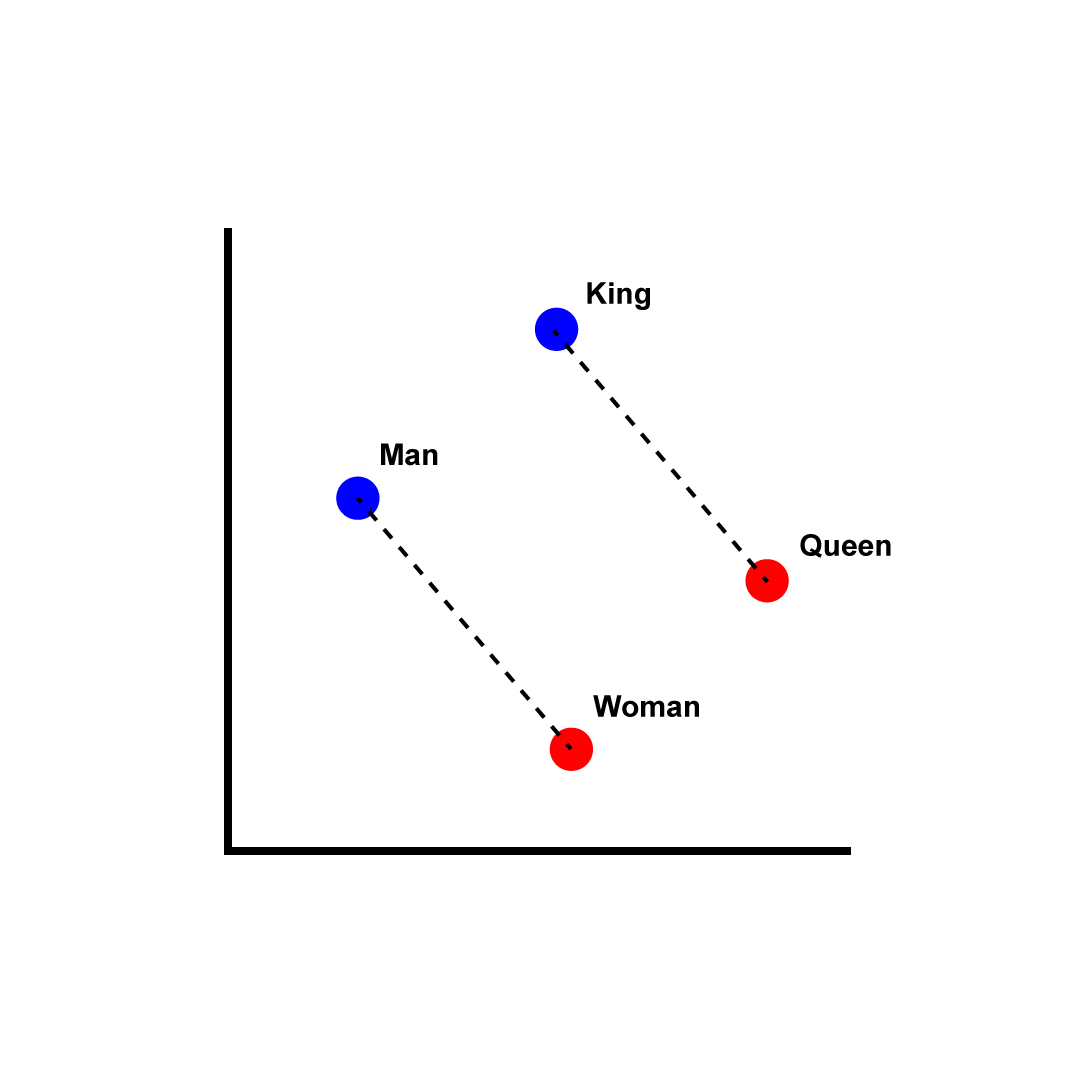
\includegraphics[scale=.2]{./images/Word_vector_illustration.jpg}
    \caption[Example of word embeddings in a semantic space.]{Description}
    \label{vector_figure}
\end{figure}

% \textit{Brunila \& LaViolette's paper revisiting the idea of distributional semantics: \url{https://arxiv.org/pdf/2205.07750.pdf} (URL for now \dots)}

\section{Word Embeddings and Co-occurrence Matrices}

Similar to the data wrangling chapter, text has to be preprocessed before the analysis. Take this sentence, for example: ``Footsteps shuffled on the stair. Under the firelight, under the brush, her hair spread out in fiery points glowed into words, then would be savagely still.'' (From T. S. Eliot's \textit{The Waste Land})

NLP generally follows this pipeline: 

- sentence segmentation

- word tokenization

- normalization and filtering

- main analysis


For sentence segmentation, the paragraph or document is segmented into sentences. This step is particularly important when using text that has been scanned using OCR, where errors might occur.
Once the document has been segmented into sentences, a tokenizer is used to split each sentence into the comprising words. 

Following tokenization, the words/tokens are generally normalized to remove capitalization or certain punctuation marks, such that the words are consistenly in the same form.
Here, stopwords (words that are deemed insignificant; usually function words) can also be filtered out.
In the above steps, the exact implementation will differ based on your research goal.

% After segmentation and tokenization: 
% [[footsteps,shuffled,on,the,stair], 
% [under,the,firelight,under,the,brush,her,hair,
% spread,out,in,fiery,points,glowed,into,words,
% then,would,be,savagely,still]] \textit{Formatting?}

After segmentation and tokenization: 
[[footsteps, shuffled, on, the, stair], 
[under, the, firelight, \dots, savagely, still]]

Once the text has been preprocessed, the main analysis can proceed. For a very basic word embedding algorithm, the label-context pair co-occurrences are tracked in a co-occurrence matrix.
Each word is iterated as the `label', while the surrounding words serve as the `context'. A window size is defined, which designates how many words to include in the `context'. Skip-gram models will include context both before and after a given label.

From our example, we may start out with ``footsteps'' as the label, then if we have a window size of two, the co-occurring label-context pairs would be [footsteps, shuffled] and [footsteps, on].
Then, when we get to ``on'' as the label, the label-context pairs would include [on, footsteps], [on, shuffled], [on, the], [on, stair].

Once the document has been processed, the result is a co-occurrence matrix where each cell represents the raw co-occurrence counts for a given label-context pair.

\textit{Make an example}.

Not every word is used with the same frequency, so some determiners (`the', `a') may be over-represented and skew the co-occurrence matrix. If these type of stopwords were not removed, we can change the weight of different contexts. Therefore, a positive-pointwise mutual information transform is often used to weight the matrix. 
\textbf{From simbrain documentation:} Weights the co-occurrence values to avoid word-frequency-bias in embeddings. Words like ``the'' and ``a'' that should not be considered meaningful in terms of co-occurrence are down-weighted. Less frequent words on the other, like ``platitude'' or ``espresso'', that are more meaningful in terms of co-occurrences, are up-weighted.

\textbf{Quote from Lenci:} PPMI measures how much the probability of a target-context pair estimated in the training corpus is higher than the probability we should expect if the target and the context occurred independently of one another. (Lenci, 2018)

\textit{See Lenci review paper for in-depth explanation and discussion.}

The result is a set of \textit{n}-dimensional vectors for a set of words, which are referred to as ``word embeddings.''

\subsection{Evaluation}

How then should these embeddings be evaluated? 
Previous research on word similarity and relatedness has shown that directly asking for relatedness judgements can accurately capture word relations (Finkelstein et al. 2002).
Therefore, the general method of evaluation is by collecting a set of human judgements, which theoretically serve as the ceiling of model of model performance. \textit{Check paper that reviewer mentioned? https://aclanthology.org/2022.bionlp-1.26/}

There are a variety of gold standards that have been used across the field, such as WordSim-353 or MEN (citations), however, recent models have already reached or surpassed human performance on these tasks.
Therefore, Hill and colleagues set out to create a gold standard that separates similarity from association, which previous standards had ignored the distinction.
For example, ``car'' and ``tire'' would be considered associated but not similar, ``glasses'' and ``spectacles'' would be considered similar. See Hill et al., 2014 for an in-depth discussion.

\subsection{Different spins}
Paragram embeddings.
Counterfitting / retrofitted embeddings.
Multilingual embeddings.
Different associative models (e.g., Mike Jones' BEAGLE).
Co-occurrence vs next-word prediction.
Multimodality.
Context-dependent transformer models.

\subsection{Corpus quality}

While different algorithms may improve the model performance and similarity to our own semantic representations, the corpus quality also has an impact on model performance.
Larger training corpora generally improve the quality of the derived embeddings. 
GloVe embeddings are trained on various trainint corpora, varying from 1 billion tokens to 42 billion tokens (from the Common Crawl) \textit{Citations.}
Beside the amount or size of the training corpora, the type of documents is also important; training solely on works of fiction would lead to different embeddings than a model trained on non-fiction, and so on. It is important to consider the meaning you are trying to capture (generalized or specific to a field, such as medical documents).

\section{Applications}
Word similarity -> cosine similarity.
Discourse tracking.
Machine translation.
Sentiment analysis.
Language change (HistWords).

\section{Shortcomings}
Polysemy and context.
Dimensionality of representations.

\section{Theoretical implications?}
Points from Boleda paper: semantic change, polysemy and composition, and the grammar-semantics interface.
\textit{Separate from shortcomings or combine these two?}

\section{Trajectory of the field}
Improvements over the years (skip-gram, counterfitting, etc.).
Transition to Language Models?

\section{Exercises}

\subsection{Basic NLP}

\begin{enumerate}
\item Walkthrough a simple example of counting co-occurrences.
\item How does window size impact the embeddings?
\item What is potential motivation for using the \textit{skip-gram} setting?
\item Calculate the similarity between these words: [list of words]. 
\item Something about the PPMI transformation?
\end{enumerate}

\subsection{Geometric thinking}

\begin{enumerate}
\item What does it mean for a word embedding to be n-dimensional?
\item Why is cosine similarity used over other distance functions, like traditional euclidean distance?
\item Something where they perform clustering?
\end{enumerate}

\subsection{Corpus quality}

\begin{enumerate}
\item With the limited (demo) training corpus, how well do you think it captures the actual meaning of the words?
\item Does corpus size or quality matter? (Too basic of a question.)
\item Something with a corpus that deals with polysemy (financial institution \& geographic texts)
\end{enumerate}

\subsection{Neural Networks and other advances}

\begin{enumerate}
\item SRNs?
\item Next-word prediction?
\item Text generation?
\end{enumerate}